\documentclass[conference,a4paper]{IEEEtran}
\usepackage[utf8]{inputenc}
\usepackage[T1]{fontenc}
\usepackage{cite}
\usepackage{amsmath,amssymb}
\usepackage{graphicx}
\usepackage{booktabs}
\usepackage{url}
\usepackage{listings}
\usepackage{textcomp}
\def\BibTeX{{\rm B\kern-.05em{\sc i\kern-.025em b}\kern-.08em T\kern-.1667em\lower.7ex\hbox{E}\kern-.125em X}}
\lstset{basicstyle=\ttfamily\scriptsize,breaklines=true,columns=fullflexible,frame=single}
\newcommand{\repourl}{\url{https://github.com/RamGhadiyaram/calibrated-stacked-credit-risk}}

\begin{document}
\title{Calibration, Not Accuracy: What Stacking Adds to Gradient Boosting in Credit Risk Scoring}
\author{\IEEEauthorblockN{Ram Ghadiyaram}
\IEEEauthorblockA{\textit{Independent Researcher}\\
Celina, TX, USA\\
\textit{Corresponding author}\\
ram.ghadiyaram@gmail.com\\
ORCID 0009-0006-3730-0914}
\and
\IEEEauthorblockN{Vishnuvardhan Peddapaidi}
\IEEEauthorblockA{\textit{Independent Researcher}\\
Plano, TX, USA\\
vishnuvardhan.peddapaidi@gmail.com\\
ORCID 0009-0006-5463-6129}
\and
\IEEEauthorblockN{Sashi Kiran Kaata}
\IEEEauthorblockA{\textit{Independent Researcher}\\
Glendale, AZ, USA\\
sashikiran9@gmail.com\\
ORCID 0009-0002-7980-2905}}

\maketitle
\begin{abstract}
Stacked ensembles are often proposed for credit risk scoring, but their benefit over a well-tuned gradient-boosted model is rarely tested with paired statistics, and the probabilities they produce are seldom audited for calibration or group fairness. We benchmark a calibrated stack of six base learners (logistic regression, XGBoost, LightGBM, CatBoost, TabNet and an FT-Transformer) against each of them on the South German Credit data and a 30,000-row sample of the Taiwan credit-card default data. We use repeated, nested cross-validation, the Nadeau-Bengio corrected $t$-test with Holm adjustment, and report discrimination, calibration, an approve-the-safest-90\% loss measure, group fairness gaps and a stylized stress sensitivity. The stack reaches an AUC of 0.795 on the German data and 0.785 on the Taiwan data. It does not beat CatBoost on either: the AUC differences are $-0.003$ and $+0.002$, and neither survives Holm adjustment. On the Taiwan data the stack lowers the Brier score by 0.0004 relative to CatBoost (Holm $p=0.032$), a gain too small to change a lending decision. The stack and CatBoost both clearly outperform TabNet, and on German data the stack's calibration slope (1.05) is closer to one than CatBoost's (0.83). Fairness gaps at 80\% approval are nearly identical across models, so model choice does not remove them. We conclude that, on these data, gradient boosting is the safer default and stacking is justified mainly by calibration stability. Code, data loaders and a verification script reproduce every number.
\end{abstract}
\begin{IEEEkeywords}
credit risk, stacked generalization, probability calibration, tabular deep learning, algorithmic fairness
\end{IEEEkeywords}

\section{Introduction}
Lenders turn applicant records into a probability of default, and that probability drives approval, pricing and capital. Three properties matter in practice. The model must rank applicants well. Its probabilities must be accurate, because they feed pricing and provisioning rather than only a cutoff \cite{vancalster,r28}. And its errors must not fall unevenly on protected groups \cite{hardt,kozodoi}. Supervisory guidance on model risk asks lenders to show evidence on all three \cite{r19,r20}.

Two claims are common in the applied literature. The first is that an ensemble of heterogeneous models, combined by stacked generalization \cite{r5}, beats any single member. The second is that deep tabular architectures such as TabNet \cite{tabnet} and the FT-Transformer \cite{ftt} are competitive with, or better than, gradient-boosted trees. The evidence for both is mixed. Large benchmarks find that tree ensembles remain hard to beat on typical tabular data \cite{r30,szarmon}, and credit scoring benchmarks find that the gap between strong classifiers is small \cite{lessmann}. Yet many credit studies report a single train-test split, no paired test, and no calibration or fairness analysis, so a gain of a few thousandths of AUC is easily mistaken for progress.

This paper asks a narrow question and answers it with care: \emph{when is a calibrated stack worth deploying over its best single member?} Our contributions are as follows.
\begin{enumerate}
\item A benchmark of a calibrated stack against six strong baselines, including TabNet and an FT-Transformer, on two public credit datasets, using repeated nested cross-validation, the Nadeau-Bengio corrected resampled $t$-test \cite{r25} and Holm adjustment \cite{holm}.
\item A calibration analysis (Brier score, expected calibration error, calibration slope, and Platt and isotonic recalibration of the stack) and a decision-oriented loss measure.
\item A group fairness audit of the approval decision for age, foreign-worker status and sex, which shows how much of the gap is model-independent.
\item A clearly labeled stylized stress sensitivity, which reports how predicted risk and rankings move under input shifts, without claiming to forecast any macroeconomic event.
\item An honest negative result and a fully reproducible pipeline: code, a notebook and a verification script that regenerates every table in this paper from fold-level outputs.
\end{enumerate}

\begin{figure*}[t]
\centering
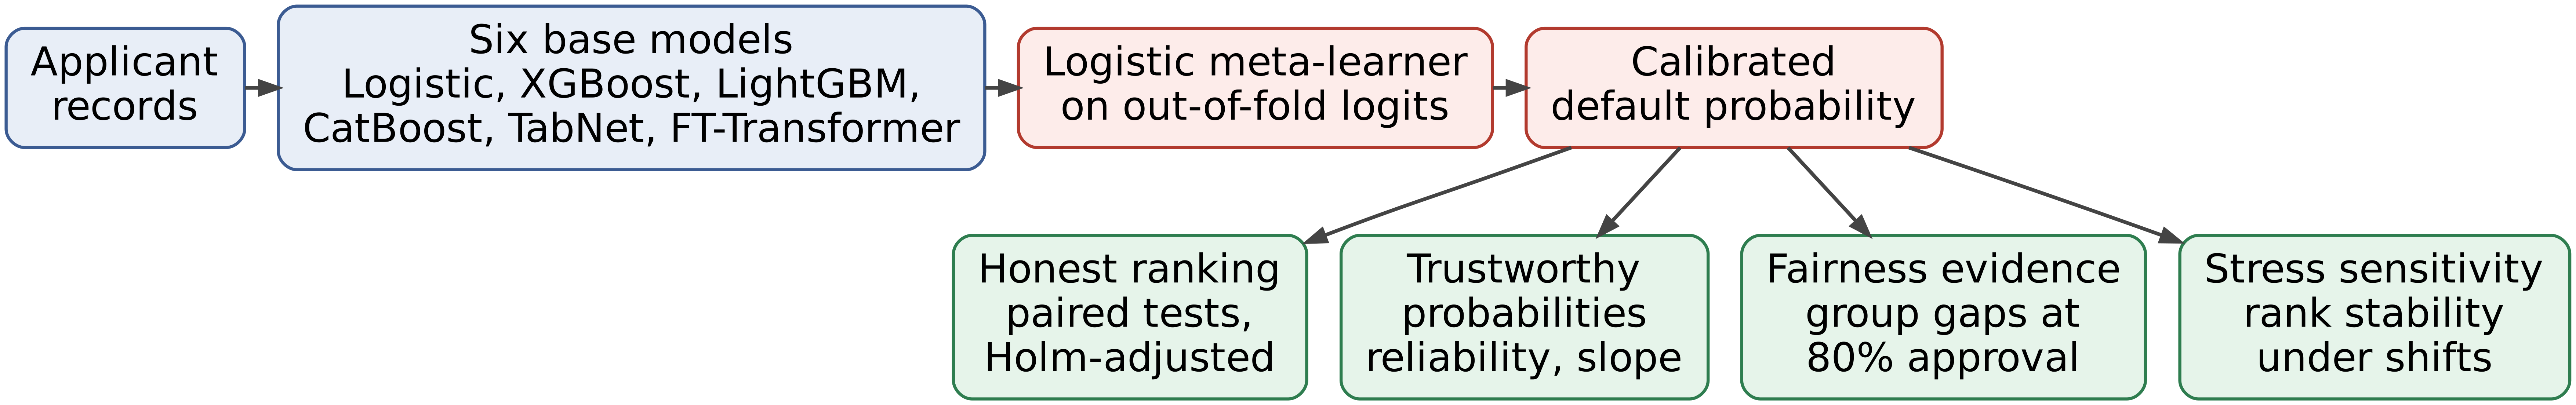
\includegraphics[width=\textwidth]{fig_framework.png}
\caption{Study design. Six base models produce out-of-fold scores, a logistic meta-learner combines them, and the resulting probability is audited for ranking, calibration, fairness and stress sensitivity.}
\label{fig:framework}
\end{figure*}

\section{Related Work}
\textbf{Credit scoring benchmarks.} Lessmann et al.\ \cite{lessmann} compared 41 classifiers on eight credit datasets and found that heterogeneous ensembles and random forests perform well and that the differences among the top methods are small. We follow their emphasis on statistical comparison, but use a paired, fold-level test that accounts for overlapping training sets \cite{r25,demsar} and add calibration and fairness.

\textbf{Gradient boosting and tabular deep learning.} XGBoost \cite{r2}, LightGBM \cite{r23} and CatBoost \cite{r24} are the default industrial choices. Grinsztajn et al.\ \cite{r30} and Shwartz-Ziv and Armon \cite{szarmon} report that trees are still strong on medium-sized tabular data, while TabNet \cite{tabnet} and the FT-Transformer \cite{ftt} are the most cited deep alternatives. We include both so that a reader does not need to ask whether a deep model would have changed the conclusion.

\textbf{Stacking and calibration.} Stacked generalization \cite{r5} fits a meta-learner on out-of-fold predictions. Probability quality is separate from ranking quality: boosted trees can be miscalibrated \cite{r32}, neural networks often are \cite{r28}, and Platt scaling \cite{r26} and isotonic regression \cite{r27} are the standard repairs. Calibration slope and calibration-in-the-large give a more informative view than a single binned error \cite{vancalster,r29}.

\textbf{Fairness in credit.} Equal opportunity \cite{hardt} compares approval rates among applicants who would repay. Kozodoi et al.\ \cite{kozodoi} study how fairness constraints interact with profit in credit scoring. We use simple, auditable gap measures at a fixed approval rate, and we report them for the same predictions that produce the performance tables.

\section{Study Design}
\subsection{Data}
Table~\ref{tab:data} summarizes the two datasets. The South German Credit data \cite{r21} is the corrected version of the Statlog German Credit data \cite{r17,r22}, with 1{,}000 applicants and a 30\% default rate. The Taiwan data \cite{r31,r33} holds 30{,}000 credit-card clients from 2005 with a 22\% default rate. We use all 30{,}000 rows. Both datasets are public and old, which limits what they can say about today's applicants (Section~\ref{sec:limits}). We derive the protected indicators as follows. For German data, \emph{age under 25} (150 applicants) and \emph{foreign worker} (963 applicants; only 37 are not foreign workers). For Taiwan data, \emph{age under 25} (2{,}685 clients) and \emph{female} (18{,}112 clients). The protected attributes remain among the model inputs, as in the original datasets, and are also used to define the audit groups; we did not remove them, so the audit describes models that can see them.

\begin{table}[t]
\centering
\caption{Datasets.}
\label{tab:data}
\small
\setlength{\tabcolsep}{3pt}
\begin{tabular}{lcccc}
\toprule
Dataset & Rows & Feat. & Default & Era\\
\midrule
German credit & 1{,}000 & 20 & 30\% & 1973--1975\\
Taiwan card & 30{,}000 & 23 & 22\% & 2005\\
\bottomrule
\end{tabular}
\end{table}

\subsection{Models and stacking}
The base learners are logistic regression, XGBoost, LightGBM, CatBoost, TabNet and an FT-Transformer implemented in PyTorch. The two stacks are \emph{Stack-GBM}, built from the logistic model and the three gradient-boosted models, and \emph{Stack-All}, which adds TabNet and the FT-Transformer. For each outer training set, we generate out-of-fold predictions for every base learner with an inner 5-fold split, convert them to logits, and fit a logistic regression meta-learner on those logits. The base learners are then refit on the full outer training set for prediction on the held-out fold. We also evaluate Platt and isotonic recalibration of the stack's output, fitted on the same out-of-fold predictions.

\subsection{Evaluation protocol}
We use repeated stratified 5-fold cross-validation as the outer loop, with three repeats on the German data (15 folds) and two on the Taiwan data (10 folds). All preprocessing, base learning, stacking and recalibration are fitted inside the outer training set, so no information from a test fold reaches training.

\subsection{Metrics}
\textbf{Discrimination:} ROC-AUC and PR-AUC. \textbf{Probability quality:} Brier score, expected calibration error (ECE, 10 equal-width bins), and the calibration slope, which is the coefficient from regressing the outcome on the logit of the predicted probability (one is ideal; below one means over-confident). \textbf{Decision loss:} the share of defaults avoided when the safest 90\% of applicants are approved, relative to approving everyone (``loss reduction''). \textbf{Fairness:} at a fixed approval rate of 80\%, the approval gap (unprivileged minus reference group) and the good-payer gap, which is the same difference restricted to applicants who did not default, an equal-opportunity style measure \cite{hardt}. We also report the observed default rate of each group, since a group with a higher true default rate will be approved less often by any accurate model.

\subsection{Statistical comparison}
Fold-level differences between Stack-All and each of the seven comparators are tested with the Nadeau-Bengio corrected resampled $t$-test \cite{r25}, which inflates the variance by a factor $(1/J + n_{\mathrm{test}}/n_{\mathrm{train}})$ for $J$ folds to account for overlapping training sets. With five-fold splitting, $n_{\mathrm{test}}/n_{\mathrm{train}}=0.25$. We adjust the seven $p$-values with Holm's procedure \cite{holm} separately for each dataset and metric.

\subsection{Stylized stress sensitivity}
We do not have real tariff or macroeconomic exposure data for these applicants, so we do not claim a tariff study. Instead we apply a transparent input shift and measure how the fitted models respond, leaving all labels unchanged. On the German data, the credit amount is multiplied by $(1+s)$. On the Taiwan data, the six repayment-amount features are reduced by a factor of $(1-s)$ and the six bill-amount features are increased by $(1+s)$. The severity $s$ takes the values 0.1, 0.2 and 0.3. We report the mean increase in predicted default probability and the Spearman rank correlation between stressed and unstressed predictions. This is a sensitivity analysis of the model, not a forecast of defaults.

\section{Results}
\subsection{Discrimination and probability quality}
Table~\ref{tab:main} reports the main results. On the Taiwan data, every strong model reaches an AUC between 0.778 and 0.785, and the stacks sit at the top: Stack-All has 0.785 and Stack-GBM 0.784, against 0.783 for CatBoost and XGBoost. Logistic regression is clearly worse at 0.724, and TabNet is intermediate at 0.765. The calibration of all tree-based models and both stacks is good, with ECE near 0.010 to 0.012 and slopes within a few hundredths of one. On the German data, CatBoost is nominally best at 0.799, with the stacks at 0.796 and 0.795. TabNet performs poorly at 0.641, which is not surprising for a model that normally needs more than 1{,}000 rows, and the FT-Transformer is at 0.740.

\begin{table*}[t]
\centering
\caption{Out-of-fold performance (mean over outer folds). German: 15 folds (3 repeats of 5-fold); Taiwan: 10 folds (2 repeats of 5-fold, 30,000 rows). Best value per column in bold; ties within rounding are all bold.}
\label{tab:main}
\small
\setlength{\tabcolsep}{3.5pt}
\begin{tabular}{l|cccc|cccc}
\toprule
 & \multicolumn{4}{c|}{South German Credit} & \multicolumn{4}{c}{Taiwan credit-card default}\\
Model & AUC & Brier & ECE & Slope & AUC & Brier & ECE & Slope\\
\midrule
Logistic & 0.782 & 0.168 & 0.086 & 0.737 & 0.724 & 0.145 & 0.050 & 0.987\\
XGBoost & 0.788 & 0.167 & 0.088 & 0.644 & 0.783 & 0.134 & 0.011 & 0.965\\
LightGBM & 0.786 & 0.168 & 0.093 & 0.627 & 0.782 & 0.134 & 0.012 & 0.961\\
CatBoost & \textbf{0.799} & \textbf{0.161} & 0.071 & 0.833 & 0.783 & 0.134 & \textbf{0.010} & 1.006\\
TabNet & 0.641 & 0.203 & 0.082 & 0.784 & 0.765 & 0.137 & 0.015 & \textbf{1.003}\\
FT-Transformer & 0.740 & 0.182 & 0.072 & 1.381 & 0.778 & 0.135 & 0.014 & 0.968\\
\midrule
Stack-GBM & 0.796 & \textbf{0.161} & \textbf{0.065} & 1.101 & 0.784 & 0.134 & \textbf{0.010} & 1.004\\
Stack-All & 0.795 & \textbf{0.161} & 0.067 & \textbf{1.048} & \textbf{0.785} & \textbf{0.133} & 0.011 & 1.004\\
\bottomrule
\end{tabular}
\end{table*}

The pattern in calibration differs from the pattern in ranking. On the German data the stack has the lowest ECE (0.065 for Stack-GBM and 0.067 for Stack-All, against 0.071 for CatBoost) and a slope of 1.05 to 1.10 against 0.83 for CatBoost and 0.63 to 0.74 for XGBoost, LightGBM and logistic regression. A slope below one indicates over-confident predictions, which is common for flexible models on small samples. The meta-learner, fitted on out-of-fold logits, corrects much of that. On the Taiwan data the sample is large enough that no model is meaningfully miscalibrated apart from logistic regression (ECE 0.050). Platt scaling of the stack changes nothing, and isotonic recalibration lowers PR-AUC (0.600 against 0.636 for Stack-All on German data, and 0.550 against 0.561 on Taiwan data), probably because the step function creates ties among scores. We therefore recommend the raw stack output.

\subsection{Paired statistical comparison}
Table~\ref{tab:paired} and Fig.~\ref{fig:paired} give the paired tests. On the German data, only the comparison with TabNet is significant after Holm adjustment, both for AUC (difference 0.155, $p_H=0.012$) and for Brier score (difference $-0.042$, $p_H=0.001$). Against CatBoost the AUC difference is $-0.003$ with an interval that comfortably spans zero. On the Taiwan data, Stack-All beats logistic regression and TabNet on both metrics ($p_H<0.001$). Against CatBoost the AUC difference of $+0.0016$ has an unadjusted $p$ of 0.028 but a Holm-adjusted $p_H$ of 0.110, so we do not claim it. For the Brier score, the stack's advantage over CatBoost ($-0.0004$, $p_H=0.032$), LightGBM ($-0.0006$, $p_H=0.013$) and Stack-GBM ($-0.0002$, $p_H=0.024$) is statistically detectable. It is also very small: the corresponding change in the loss measure is not distinguishable, with all strong models reducing losses by about 0.24 on the Taiwan data (the full metric table is in the released \texttt{results.md}).

\begin{table*}[t]
\centering
\caption{Paired differences, Stack-All minus each comparator, over outer folds. Mean difference with 95\% interval from the Nadeau-Bengio corrected resampled $t$-test; $p_H$ is the Holm-adjusted $p$-value over the seven comparators. Negative Brier differences favor Stack-All.}
\label{tab:paired}
\small
\setlength{\tabcolsep}{2pt}
\begin{tabular}{l|rcr|rcr}
\toprule
Comparator & \multicolumn{3}{c|}{AUC difference} & \multicolumn{3}{c}{Brier difference}\\
 & Diff. & 95\% interval & $p_H$ & Diff. & 95\% interval & $p_H$\\
\midrule
\multicolumn{7}{l}{\textit{South German Credit (15 folds)}}\\
Logistic & +0.0135 & [$-$0.0118,  +0.0388] & 1.000 & $-$0.0069 & [$-$0.0165,  +0.0026] & 0.424\\
XGBoost & +0.0075 & [$-$0.0100,  +0.0249] & 1.000 & $-$0.0060 & [$-$0.0128,  +0.0008] & 0.310\\
LightGBM & +0.0096 & [$-$0.0102,  +0.0293] & 1.000 & $-$0.0072 & [$-$0.0142,  $-$0.0002] & 0.228\\
CatBoost & $-$0.0034 & [$-$0.0161,  +0.0092] & 1.000 & +0.0002 & [$-$0.0049,  +0.0053] & 1.000\\
TabNet & +0.1545 & [+0.0690,  +0.2399] & 0.012 & $-$0.0417 & [$-$0.0596,  $-$0.0238] & 0.001\\
FT-Transformer & +0.0550 & [$-$0.0024,  +0.1124] & 0.355 & $-$0.0211 & [$-$0.0363,  $-$0.0059] & 0.060\\
Stack-GBM & $-$0.0006 & [$-$0.0062,  +0.0051] & 1.000 & +0.0005 & [$-$0.0017,  +0.0027] & 1.000\\
\midrule
\multicolumn{7}{l}{\textit{Taiwan credit-card default (10 folds)}}\\
Logistic & +0.0604 & [+0.0511,  +0.0698] & $<$0.001 & $-$0.0114 & [$-$0.0129,  $-$0.0099] & $<$0.001\\
XGBoost & +0.0015 & [$-$0.0007,  +0.0037] & 0.265 & $-$0.0005 & [$-$0.0009,  $-$0.0000] & 0.077\\
LightGBM & +0.0023 & [+0.0007,  +0.0039] & 0.051 & $-$0.0006 & [$-$0.0009,  $-$0.0003] & 0.013\\
CatBoost & +0.0016 & [+0.0002,  +0.0030] & 0.110 & $-$0.0004 & [$-$0.0006,  $-$0.0001] & 0.032\\
TabNet & +0.0196 & [+0.0151,  +0.0241] & $<$0.001 & $-$0.0037 & [$-$0.0046,  $-$0.0028] & $<$0.001\\
FT-Transformer & +0.0066 & [$-$0.0012,  +0.0143] & 0.265 & $-$0.0015 & [$-$0.0031,  +0.0000] & 0.077\\
Stack-GBM & +0.0005 & [$-$0.0002,  +0.0012] & 0.265 & $-$0.0002 & [$-$0.0003,  $-$0.0001] & 0.024\\
\bottomrule
\end{tabular}
\end{table*}

\begin{figure*}[t]
\centering
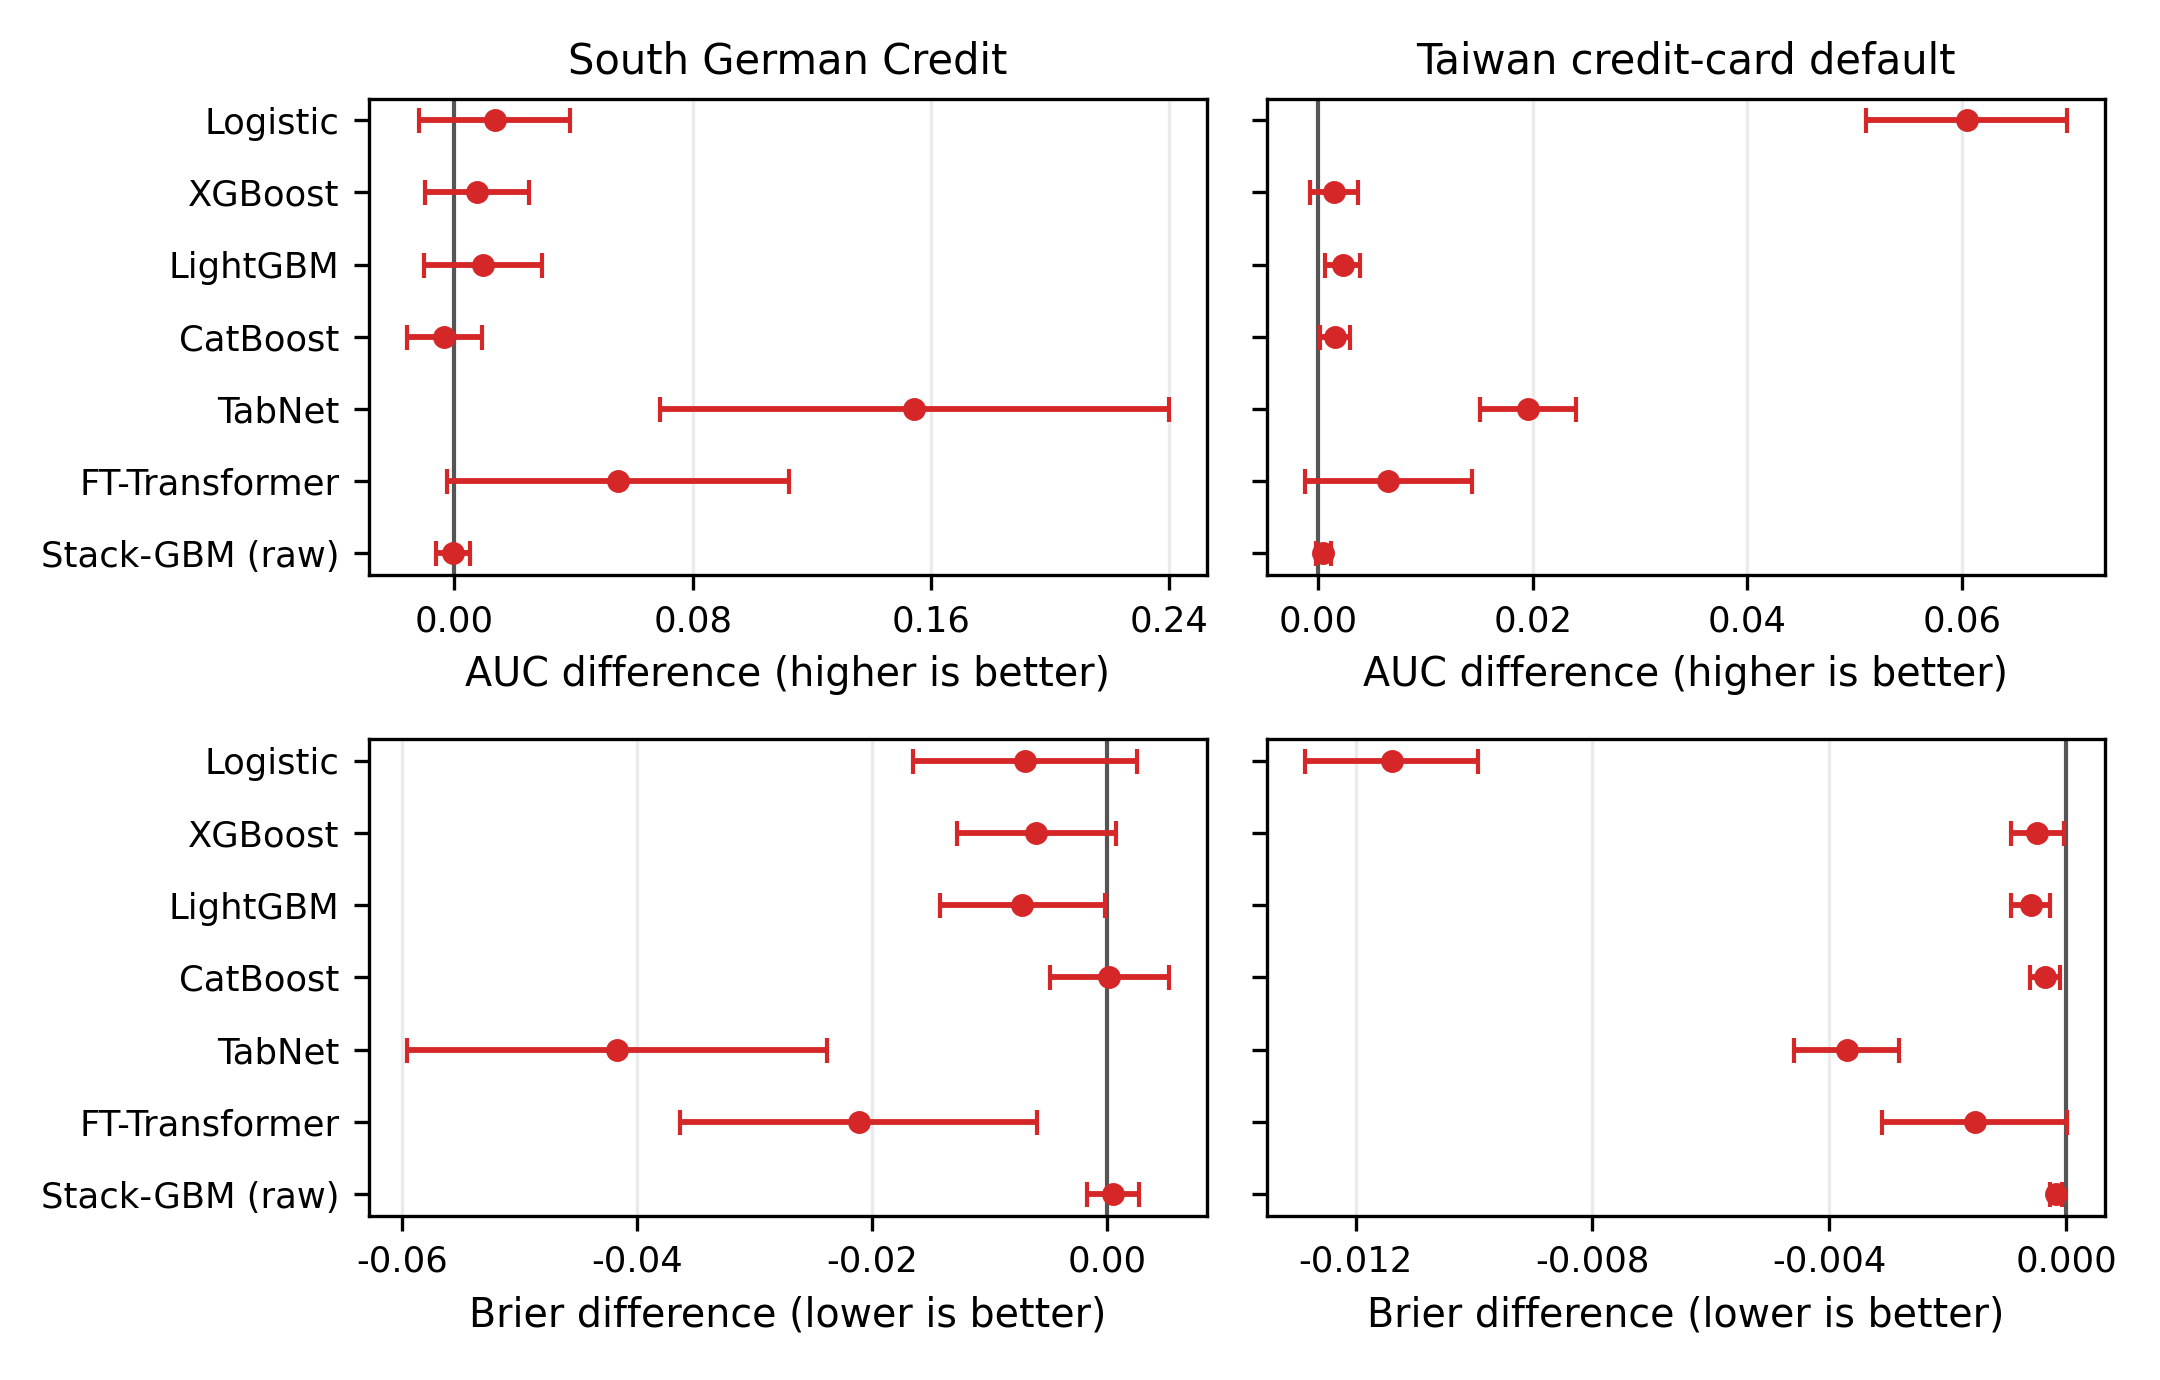
\includegraphics[width=\textwidth]{fig_paired.png}
\caption{Stack-All minus each comparator, with 95\% Nadeau-Bengio intervals (before Holm adjustment). For AUC, points to the right of zero favor the stack; for Brier score, points to the left do.}
\label{fig:paired}
\end{figure*}

\begin{figure*}[t]
\centering
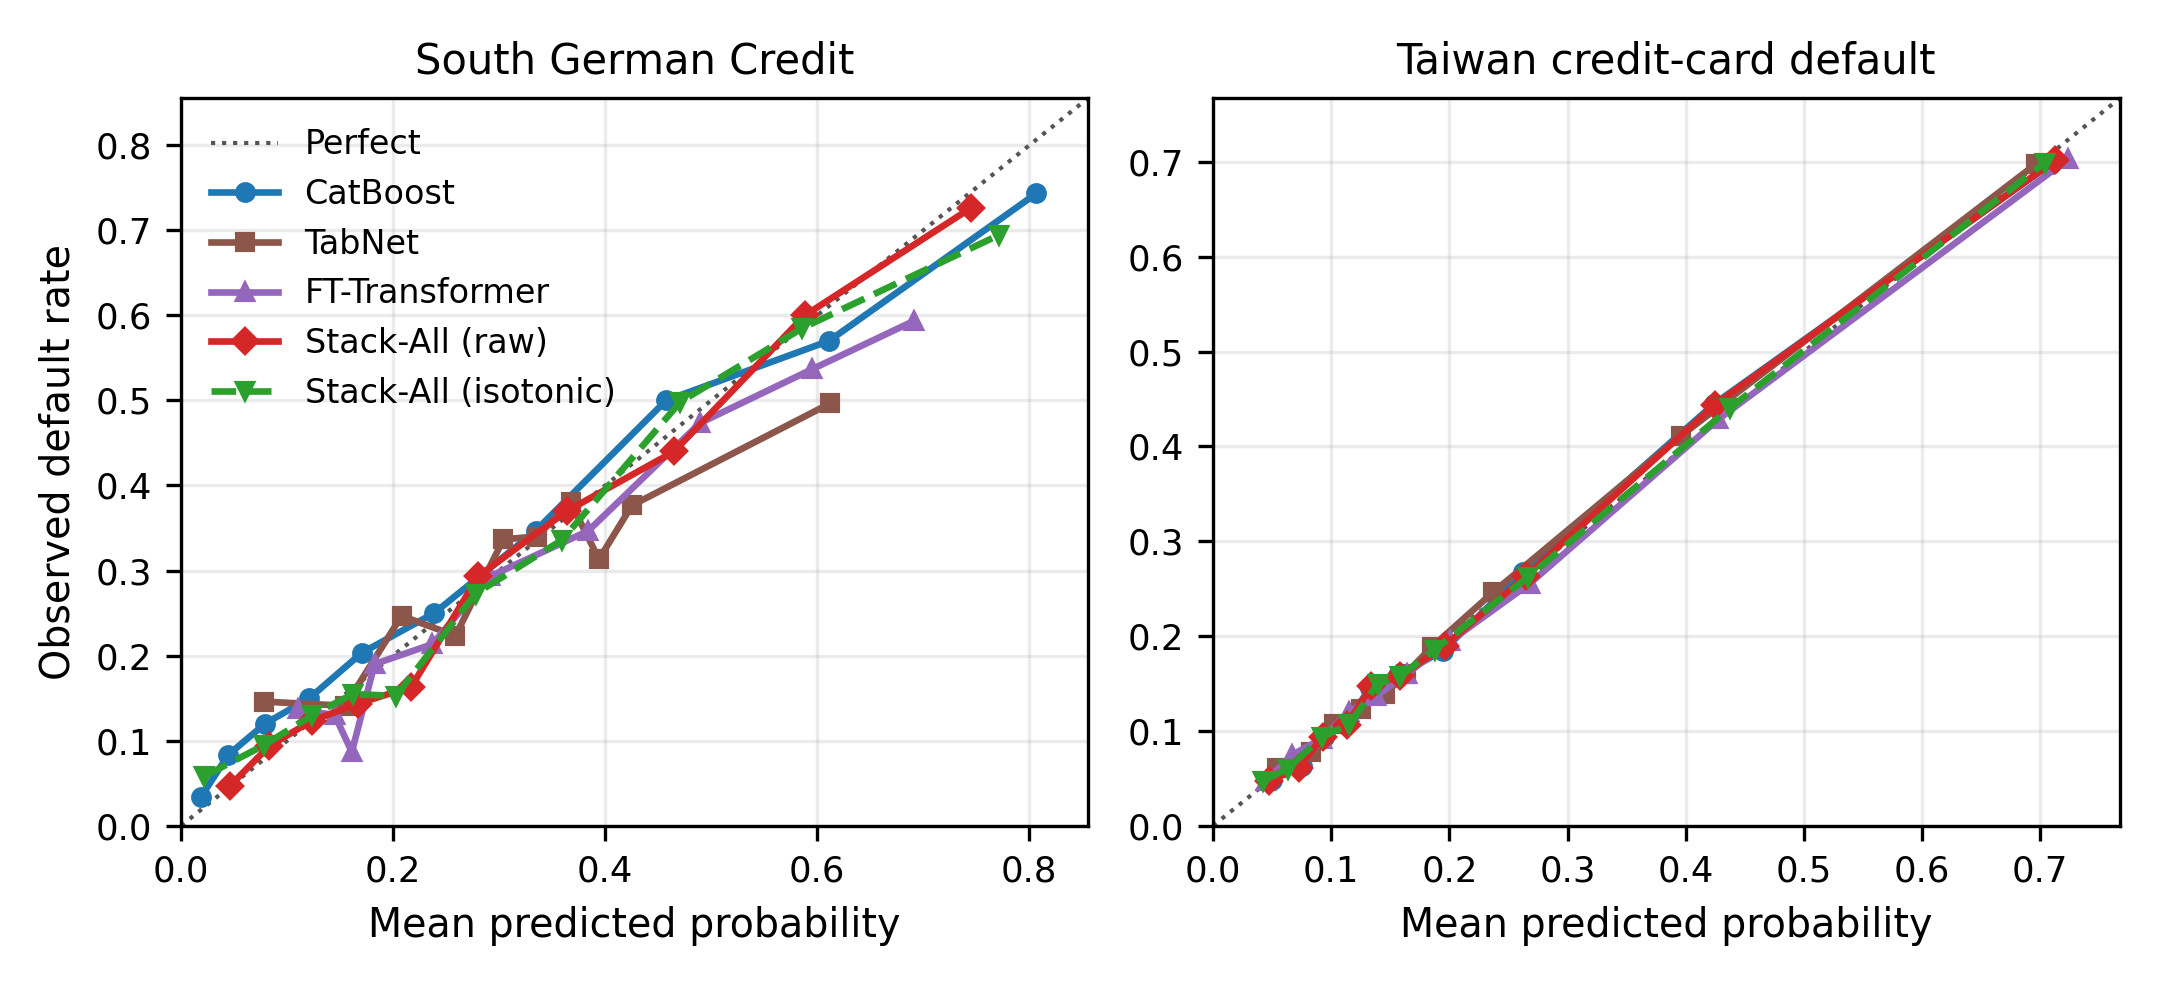
\includegraphics[width=\textwidth]{fig_reliability.png}
\caption{Reliability diagrams from pooled out-of-fold predictions. Each marker is a decile of predicted risk. Points on the dotted diagonal are perfectly calibrated.}
\label{fig:reliability}
\end{figure*}

Fig.~\ref{fig:reliability} shows the corresponding reliability diagrams. On the Taiwan data the curves overlap the diagonal for CatBoost, the FT-Transformer and the stack. On the German data all curves are noisy because of the small sample.

\subsection{Fairness audit}
Table~\ref{tab:fair} shows the audit at 80\% approval. Two points stand out. First, the gaps are large and similar for all models. On the German data, applicants under 25 are approved 14 to 16 percentage points less often than older applicants, and their observed default rate is 41\% against 28\%. On the Taiwan data, clients under 25 are approved 5.5 to 7.5 points less often (observed default 27\% against 22\%), and women are approved 5 to 6 points \emph{more} often (observed default 21\% against 24\%). In each case the direction follows the observed default rate, which means the gap is driven by the data and not by a particular model. Second, moving from logistic regression to CatBoost or the stack does not remove the gap, and in some rows increases it slightly, plausibly because a more accurate model follows the groups' true risk differences more closely. The foreign-worker comparison on the German data is unreliable because the reference group has 37 applicants, and we do not draw conclusions from it. We note that the gap for age is a statistical association and not a statement of legal or ethical acceptability; whether age may be used at all is a policy question \cite{r20}.

\begin{table}[t]
\centering
\caption{Fairness audit at 80\% approval. Gaps are the unprivileged group minus the reference group (mean over folds). Approval gap: share approved. Good-payer gap: share of non-defaulters approved. Observed default rate of each group shown for context. DE is South German Credit and TW is Taiwan; the number in brackets is the size of the unprivileged group. The German foreign-worker reference group has only 37 applicants, so that gap is noisy.}
\label{tab:fair}
\small
\setlength{\tabcolsep}{1.5pt}
\begin{tabular}{@{}llcccc@{}}
\toprule
Group & Model & Approval & Good-payer & \multicolumn{2}{c}{Default rate}\\
 & & gap & gap & Unpriv. & Ref.\\
\midrule
DE age $<$25 (150) & Logistic & $-$0.143 & $-$0.141 & 41.3\% & 28.0\%\\
 & CatBoost & $-$0.163 & $-$0.133 & 41.3\% & 28.0\%\\
 & Stack-All & $-$0.152 & $-$0.129 & 41.3\% & 28.0\%\\
\midrule
DE foreign (963) & Logistic & $-$0.190 & $-$0.104 & 30.7\% & 10.8\%\\
 & CatBoost & $-$0.084 & $-$0.023 & 30.7\% & 10.8\%\\
 & Stack-All & $-$0.148 & $-$0.070 & 30.7\% & 10.8\%\\
\midrule
TW age $<$25 (2685) & Logistic & $-$0.055 & $-$0.024 & 27.2\% & 21.6\%\\
 & CatBoost & $-$0.072 & $-$0.044 & 27.2\% & 21.6\%\\
 & Stack-All & $-$0.074 & $-$0.044 & 27.2\% & 21.6\%\\
\midrule
TW female (18112) & Logistic & +0.061 & +0.046 & 20.8\% & 24.2\%\\
 & CatBoost & +0.053 & +0.036 & 20.8\% & 24.2\%\\
 & Stack-All & +0.055 & +0.037 & 20.8\% & 24.2\%\\
\bottomrule
\end{tabular}
\end{table}

\subsection{Stylized stress sensitivity}
Table~\ref{tab:stress} reports the response to the severity-0.3 shift. On the Taiwan data the average predicted default probability rises by 0.3 percentage points for logistic regression, 2.0 for XGBoost, 2.3 for LightGBM, 1.3 for CatBoost and 1.6 for Stack-All, which means flexible models react more strongly to the same input shift than a linear model does. The stack lies between the linear model and the most reactive boosted models. Rank correlation with the unstressed ordering stays at 0.93 or higher for every model on both datasets, so the ordering of applicants is stable even when the level of risk moves. Because the shifted inputs are not tied to observed outcomes, we interpret these numbers only as a comparison of model sensitivity, not as expected default under a macroeconomic scenario.

\begin{table}[t]
\centering
\caption{Stylized stress sensitivity at severity 0.3: mean increase in predicted default probability (percentage points) and Spearman rank correlation with the unstressed ranking. Labels are unchanged; this is not a tariff forecast.}
\label{tab:stress}
\small
\setlength{\tabcolsep}{4pt}
\begin{tabular}{l|cc|cc}
\toprule
 & \multicolumn{2}{c|}{German} & \multicolumn{2}{c}{Taiwan}\\
Model & Uplift & Rank $\rho$ & Uplift & Rank $\rho$\\
\midrule
Logistic & 1.78 & 0.998 & 0.33 & 0.997\\
XGBoost & 0.09 & 0.948 & 2.03 & 0.946\\
LightGBM & 0.16 & 0.937 & 2.25 & 0.941\\
CatBoost & 0.23 & 0.966 & 1.31 & 0.980\\
TabNet & 0.35 & 0.944 & 0.53 & 0.974\\
FT-Transformer & 0.18 & 0.993 & 1.56 & 0.974\\
Stack-GBM & 0.54 & 0.973 & 1.61 & 0.972\\
Stack-All & 0.47 & 0.976 & 1.63 & 0.973\\
\bottomrule
\end{tabular}
\end{table}

\section{Discussion}
\textbf{What the stack buys.} The stack does not improve ranking over CatBoost in a way that survives correction for multiple comparisons. What it does offer is stability: on the small German sample its calibration slope is near one, whereas XGBoost, LightGBM and CatBoost are over-confident, and on the larger Taiwan sample it delivers the smallest Brier score by a margin that is statistically detectable but economically negligible. A lender who values a single, stable probability across portfolio sizes may accept the added cost. A lender who values simplicity should deploy CatBoost.

\textbf{What deep tabular models add.} On these data, TabNet and the FT-Transformer do not help. TabNet is clearly worse on both datasets, and the FT-Transformer is competitive only on the larger one. Including them in the stack did not change the result: Stack-All and Stack-GBM differ by 0.001 AUC or less.

\textbf{Practical guidance.} (1) Use a gradient-boosted model as the default and test any proposed ensemble against it with a corrected paired test. (2) Report calibration slope, not only AUC, since the stack's main advantage appears there. (3) Do not recalibrate a logistic stack with isotonic regression. (4) Audit approvals at the operating point, and compare the gap with the groups' observed default rates before attributing it to the model.

\section{Limitations}\label{sec:limits}
\textbf{Data age and scope.} The German data come from the 1970s and the Taiwan data from 2005. Neither reflects current products, bureaus or regulation, and we could not obtain a recent public dataset with applicant-level outcomes. The conclusions are about the method comparison, and may not transfer to a modern portfolio.
\textbf{No real macroeconomic exposure.} The stress analysis is a stylized input shift. A study of tariffs or other shocks requires time-stamped outcomes and exposure data, which are not available here.
\textbf{Small German sample.} With 1{,}000 rows, differences below about 0.01 AUC cannot be resolved, and the foreign-worker audit rests on 37 reference applicants.
\textbf{Taiwan subsample and tuning.} Hyperparameters are fixed at standard values and not tuned per dataset. A larger search might lift individual models, although it would also favor the baselines.
\textbf{Fairness scope.} We report two simple gap measures at one approval rate. We do not evaluate mitigation, intersectional groups or the legal admissibility of any attribute.
\textbf{Hardware.} The deep models were trained on a GPU, so small numerical differences from a CPU run are expected. The verification script checks the reported tables against the saved fold outputs, not bitwise equality of training.

\section{Conclusion}
We tested whether a calibrated stack of six learners is worth deploying over its best single member on two public credit datasets. It is not clearly better at ranking than CatBoost, and it is clearly better than TabNet and logistic regression. Its advantages are a calibration slope near one on small data and a very small but statistically detectable Brier gain on larger data. Fairness gaps are almost model-independent, and a stylized stress shows that flexible models react more strongly than a linear model while keeping the ordering of applicants nearly intact. We recommend gradient boosting as the default and the stack as an option when calibration stability matters. Future work should repeat this protocol on recent applicant-level data with real exposure variables.

\section*{Reproducibility}
The code, notebook and verification script are in the project repository, \repourl. The script \texttt{verify\_paper.py} re-derives every table from the fold-level outputs and fails if any value differs. Seeds are fixed, and the deep models can be skipped with a single flag for a CPU-only run.

\begin{thebibliography}{99}
\bibitem{r2} T. Chen and C. Guestrin, "XGBoost: A scalable tree boosting system," in Proc. 22nd ACM SIGKDD Int. Conf. Knowledge Discovery and Data Mining, San Francisco, CA, USA, 2016, pp. 785-794.
\bibitem{r5} D. H. Wolpert, "Stacked generalization," Neural Networks, vol. 5, no. 2, pp. 241-259, 1992.
\bibitem{r17} H. Hofmann, "Statlog (German Credit Data)," UCI Machine Learning Repository, 1994. [Online]. Available: \url{https://doi.org/10.24432/C5NC77}
\bibitem{r19} Board of Governors of the Federal Reserve System and Office of the Comptroller of the Currency, "SR 11-7: Supervisory guidance on model risk management," Washington, DC, USA, Apr. 2011.
\bibitem{r20} Equal Credit Opportunity Act, Regulation B, 12 C.F.R. Part 1002, 2011.
\bibitem{r21} "South German Credit," UCI Machine Learning Repository, 2020. [Online]. Available: \url{https://doi.org/10.24432/C5QG88}
\bibitem{r22} U. Groemping, "South German Credit Data: Correcting a Widely Used Data Set," Rep. 4/2019, Reports in Mathematics, Physics and Chemistry, Dept. II, Beuth Univ. of Applied Sciences Berlin, Berlin, Germany, 2019.
\bibitem{r23} G. Ke et al., "LightGBM: A highly efficient gradient boosting decision tree," in Advances in Neural Information Processing Systems (NeurIPS), vol. 30, 2017, pp. 3146-3154.
\bibitem{r24} L. Prokhorenkova, G. Gusev, A. Vorobev, A. V. Dorogush, and A. Gulin, "CatBoost: Unbiased boosting with categorical features," in Advances in Neural Information Processing Systems (NeurIPS), vol. 31, 2018, pp. 6638-6648.
\bibitem{r25} C. Nadeau and Y. Bengio, "Inference for the generalization error," Machine Learning, vol. 52, no. 3, pp. 239-281, 2003.
\bibitem{r26} J. C. Platt, "Probabilistic outputs for support vector machines and comparisons to regularized likelihood methods," in Advances in Large Margin Classifiers, A. J. Smola, P. Bartlett, B. Scholkopf, and D. Schuurmans, Eds. Cambridge, MA, USA: MIT Press, 1999, pp. 61-74.
\bibitem{r27} B. Zadrozny and C. Elkan, "Transforming classifier scores into accurate multiclass probability estimates," in Proc. 8th ACM SIGKDD Int. Conf. Knowledge Discovery and Data Mining, Edmonton, AB, Canada, 2002, pp. 694-699.
\bibitem{r28} C. Guo, G. Pleiss, Y. Sun, and K. Q. Weinberger, "On calibration of modern neural networks," in Proc. 34th Int. Conf. Machine Learning (ICML), Sydney, Australia, 2017, pp. 1321-1330.
\bibitem{r29} M. P. Naeini, G. F. Cooper, and M. Hauskrecht, "Obtaining well calibrated probabilities using Bayesian binning," in Proc. 29th AAAI Conf. Artificial Intelligence, Austin, TX, USA, 2015, pp. 2901-2907.
\bibitem{r30} L. Grinsztajn, E. Oyallon, and G. Varoquaux, "Why do tree-based models still outperform deep learning on typical tabular data?" in Advances in Neural Information Processing Systems (NeurIPS), Datasets and Benchmarks Track, vol. 35, 2022.
\bibitem{r31} I.-C. Yeh and C.-H. Lien, "The comparisons of data mining techniques for the predictive accuracy of probability of default of credit card clients," Expert Systems with Applications, vol. 36, no. 2, pp. 2473-2480, 2009.
\bibitem{r33} I.-C. Yeh, "Default of Credit Card Clients," UCI Machine Learning Repository, 2009. [Online]. Available: \url{https://doi.org/10.24432/C55S3H}
\bibitem{r32} A. Niculescu-Mizil and R. Caruana, "Predicting good probabilities with supervised learning," in Proc. 22nd Int. Conf. Machine Learning (ICML), Bonn, Germany, 2005, pp. 625-632.
\bibitem{tabnet} S. O. Arik and T. Pfister, "TabNet: Attentive interpretable tabular learning," in Proc. 35th AAAI Conf. Artificial Intelligence, vol. 35, no. 8, 2021, pp. 6679-6687.
\bibitem{ftt} Y. Gorishniy, I. Rubachev, V. Khrulkov, and A. Babenko, "Revisiting deep learning models for tabular data," in Advances in Neural Information Processing Systems (NeurIPS), vol. 34, 2021, pp. 18932-18943.
\bibitem{szarmon} R. Shwartz-Ziv and A. Armon, "Tabular data: Deep learning is not all you need," Information Fusion, vol. 81, pp. 84-90, 2022.
\bibitem{lessmann} S. Lessmann, B. Baesens, H.-V. Seow, and L. C. Thomas, "Benchmarking state-of-the-art classification algorithms for credit scoring: An update of research," European Journal of Operational Research, vol. 247, no. 1, pp. 124-136, 2015.
\bibitem{hardt} M. Hardt, E. Price, and N. Srebro, "Equality of opportunity in supervised learning," in Advances in Neural Information Processing Systems (NeurIPS), vol. 29, 2016, pp. 3315-3323.
\bibitem{holm} S. Holm, "A simple sequentially rejective multiple test procedure," Scandinavian Journal of Statistics, vol. 6, no. 2, pp. 65-70, 1979.
\bibitem{demsar} J. Demsar, "Statistical comparisons of classifiers over multiple data sets," Journal of Machine Learning Research, vol. 7, pp. 1-30, 2006.
\bibitem{kozodoi} N. Kozodoi, J. Jacob, and S. Lessmann, "Fairness in credit scoring: Assessment, implementation and profit implications," European Journal of Operational Research, vol. 297, no. 3, pp. 1083-1099, 2022.
\bibitem{vancalster} B. Van Calster, D. J. McLernon, M. van Smeden, L. Wynants, and E. W. Steyerberg, "Calibration: The Achilles heel of predictive analytics," BMC Medicine, vol. 17, art. 230, 2019.
\end{thebibliography}
\end{document}
